\documentclass[9pt]{beamer}
\usepackage[utf8]{inputenc}
\usepackage[romanian]{babel}

%\usetheme{Madrid}
\usecolortheme{default}
\def\code#1{\texttt{#1}}

%------------------------------------------------------------
%This block of code defines the information to appear in the
%Title page
\title[SmartForms API] %optional
{\emph{SmartForms API}: un framework pentru creearea \c si parsarea automat\u a a formularelor}

\subtitle{Lucrare de Licen\c t\u a}

%\author[Arthur, Doe] % (optional)
%{A.~B.~Arthur\inst{1} \and J.~Doe\inst{2}}

\author % (optional)
{Theodor-Pierre Moroianu}


\institute[Unibuc] % (optional)
{
	Facultatea de Matematic\u a-Informatic\u a\\
	Universitatea din Bucure\c sti
}

%\date[VLC 2021] % (optional)
%{Very Large Conference, April 2021}

%\logo{\includegraphics[height=1cm]{overleaf-logo}}

%End of title page configuration block
%------------------------------------------------------------



%------------------------------------------------------------
%The next block of commands puts the table of contents at the 
%beginning of each section and highlights the current section:

\AtBeginSection[]
{
	\begin{frame}
		\frametitle{Cuprins}
		\tableofcontents[currentsection]
	\end{frame}
}
%------------------------------------------------------------


\begin{document}

%The next statement creates the title page.
\frame{\titlepage}


%---------------------------------------------------------
%This block of code is for the table of contents after
%the title page
\begin{frame}
	\frametitle{Cuprins}
	\tableofcontents
\end{frame}
%---------------------------------------------------------

%%%%%%%%%%%%%%%%%%%%%%%%%%%%%%%%%%%%%%%%%%%%%%%%%%%%%%%%%%%%%%%
\section{Introducere}

\begin{frame}
	\frametitle{Functionalitatile produsului}
	
	\emph{SmartForms API} este un framework care permite manipularea formularelor.\\
	\vspace{10pt}
		
	Functionalitatile sale cheie sunt:
	
	\begin{itemize}
		\item Crearea, vizualizarea si stergerea formularelor.%\pause
		\item Completarea formularelor digital.%\pause
		\item Exportarea formularelor in format \emph{PDF}, si parsarea raspunsurilor din poze ale unor formulare imprimate si completate de mana.%\pause
		\item Autentificarea utilizatorilor.
	\end{itemize}
\end{frame}

\begin{frame}
	\frametitle{Tehnologii folosite}
	TODO
	\emph{SmartForms API} este un framework care permite manipularea formularelor.\\
	Functionalitatile sale cheie sunt:
	
	\begin{itemize}
		\item Crearea, vizualizarea si stergerea formularelor.%\pause
		\item Completarea formularelor digital.%\pause
		\item Exportarea formularelor in format \emph{PDF}, si parsarea raspunsurilor din poze ale unor formulare imprimate si completate de mana.%\pause
		\item Autentificarea utilizatorilor.
	\end{itemize}
\end{frame}

\section{Exemple de utilizare}

\begin{frame}
	\frametitle{Exemplu de utilizare 1: Examen scris}
	\begin{columns}
		\column{0.7\textwidth}
		Un profesor organizeaza un examen, cu intrebari tip grila sau cu un raspuns bine-definit.\\
		\begin{itemize}
			\item Un examen online permite frauda.
			\item Un examen scris necesita corectare manuala.
		\end{itemize}
		\vspace{10pt}
		Cu \textit{SmartForms}, profesorul:
		\begin{enumerate}
			\item Creeaza examenul ca un formular, pe care il imprima.
			\item Cere studentilor sa isi scrie raspunsurile pe care o copie a formularului.
			\item Scaneaza toate formularele si le incarca pe \textit{SmartForms}.
			\item Descarca numerizarea acestora, in format \code{CSV} sau \code{XLSX}.
		\end{enumerate}
		\column{0.3\textwidth}
		\begin{figure}[!h]
			\centering
			\fbox{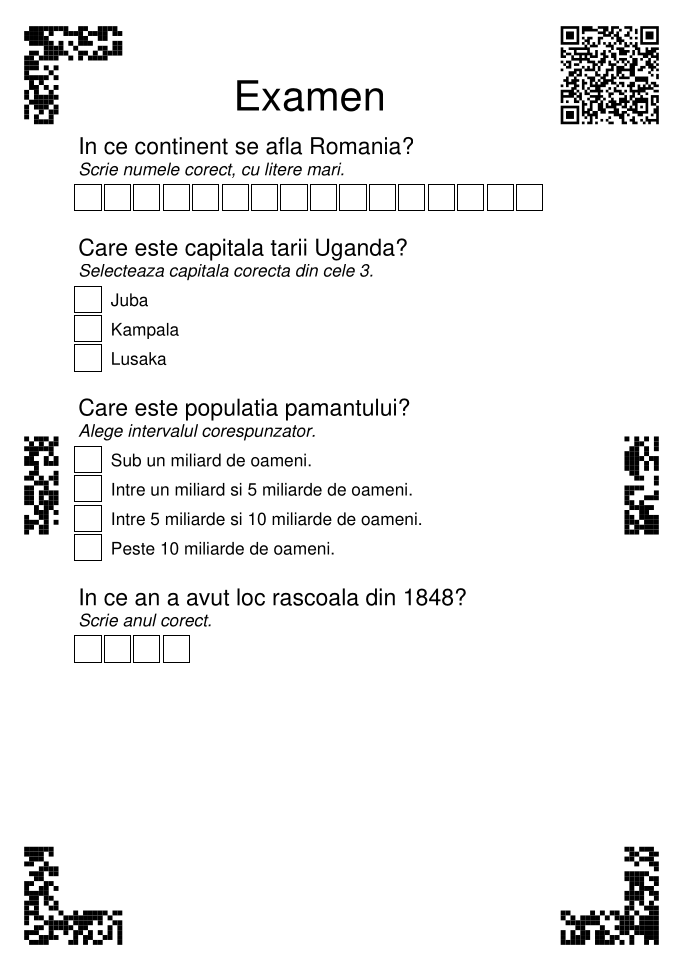
\includegraphics[height=4cm]{images/sample-forms/sample-exam.png}}
		\end{figure}
	\end{columns}
\end{frame}

\begin{frame}
	\frametitle{Exemplu de utilizare 2: Chestionar medical}
	\begin{columns}
		\column{0.7\textwidth}
		Majoritatea spitalelor si a clinicilor cer pacientilor sa completeze chestionare medicale. Dupa ce sunt completate de pacienti, acestea sunt transcrise manual in sistemul informatic al institutiei.\\
		\vspace{10pt}
		Cu \textit{SmartForms}, procesul de-a copia datele pacientilor din format fizic in format digital este automatizat:
		\begin{enumerate}
			\item Un formular cu intrebarile necesare este creeat pe \textit{SmartForms}, si descarcat ca document \textit{PDF}.
			\item Pacientii sunt rugati sa completeze formularul.
			\item Formularul este scanat si incarcat pe \textit{SmartForms}, care extrage si salveaza automat datele.
		\end{enumerate}
		\column{0.3\textwidth}
		\begin{figure}[!h]
			\centering
			\fbox{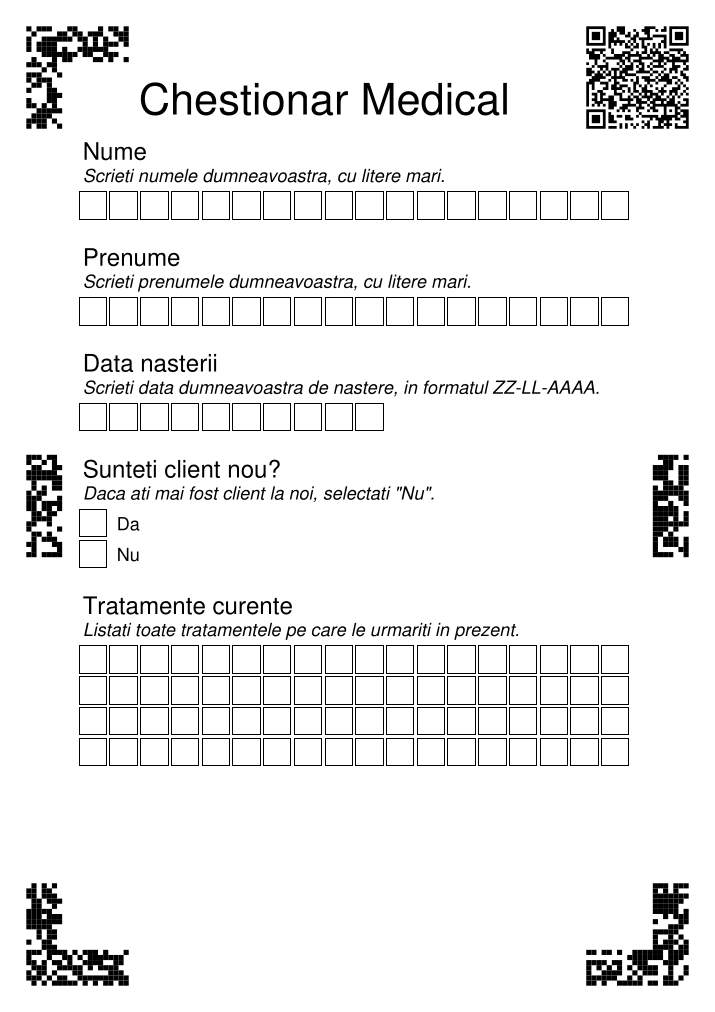
\includegraphics[height=4cm]{images/sample-forms/sample-chestionar-medical.png}}
		\end{figure}
	\end{columns}
\end{frame}

\begin{frame}
	\frametitle{Exemplu de utilizare 3: Petitii pe strada}
	\begin{columns}
		\column{0.7\textwidth}
		Un grup de voluntari doreste sa stranga datele de contact ale oamenilor interesati de o anumita tematica. Procesul standard este de-a strange datele oamenilor pe formulare, care sunt transcrise manual pe un calculator.\\
		\vspace{10pt}
		Cu \textit{SmartForms}, voluntarii pot creea si exporta ca \textit{PDF} formularele, si pot incarca scanuri ale formularelor completate, care sunt parsate automat.
		\column{0.3\textwidth}
		\begin{figure}[!h]
			\centering
			\fbox{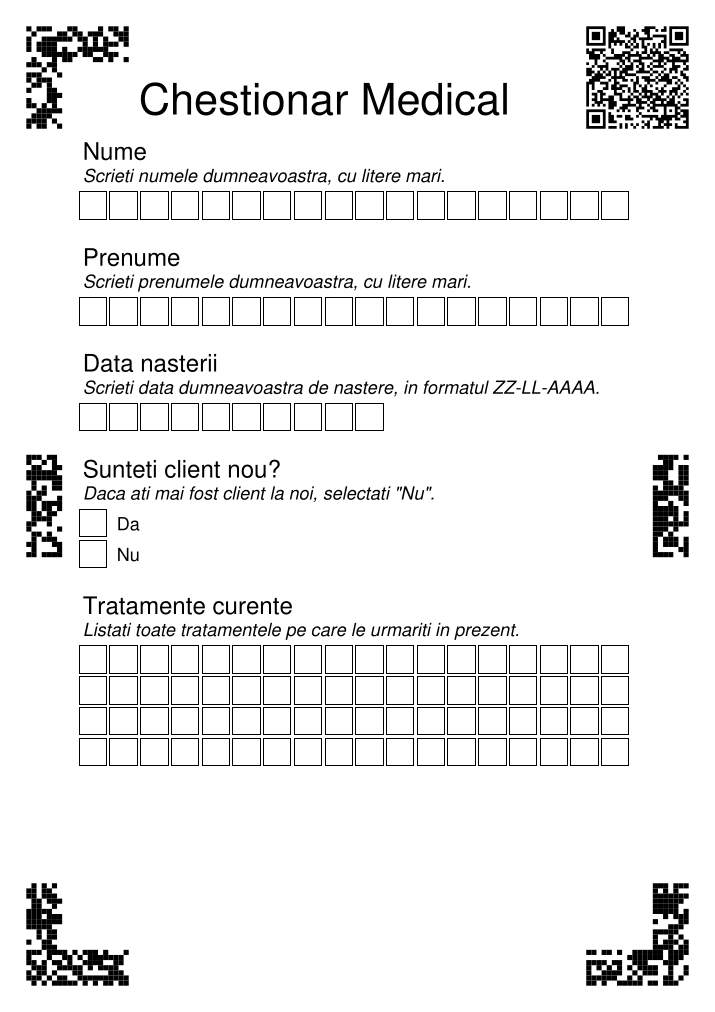
\includegraphics[height=4cm]{images/sample-forms/sample-chestionar-medical.png}}
		\end{figure}
		TODO: Alt formular
	\end{columns}
\end{frame}


\begin{frame}
	\frametitle{Exemplu de utilizare 4: Protectia datelor personale}
	O organizatie doreste sa foloseasca o aplicatie de gestionare a formularelor. Aplicatii online precum \textit{Google Forms} sunt intr-o zona gri din punct de vedere a GDPR-ului, si folosirea acestora necesita diferite proceduri legale.\\
	\vspace{10pt}
	Cum \textit{SmartForms} poate fi gazduit local, datele personale ale utilizatorilor nu parasesc serverele organizatiei, care poate folosi framework-ul ca si cum ar fi unul produs intern, al carui date nu trec print-un serviciu tert (third-party service).
			
\end{frame}



%Two columns
\begin{frame}
	\frametitle{Two-column slide}
	
	\begin{columns}
		
		\column{0.5\textwidth}
		This is a text in first column. df fd df f
		$$E=mc^2$$
		\begin{itemize}
			\item First item
			\item Second item
		\end{itemize}
		
		\column{0.5\textwidth}
%		This text will be in the second column
%		and on a second tought this is a nice looking
%		layout in some cases.
		
		
		\begin{figure}[!h]
			\centering
			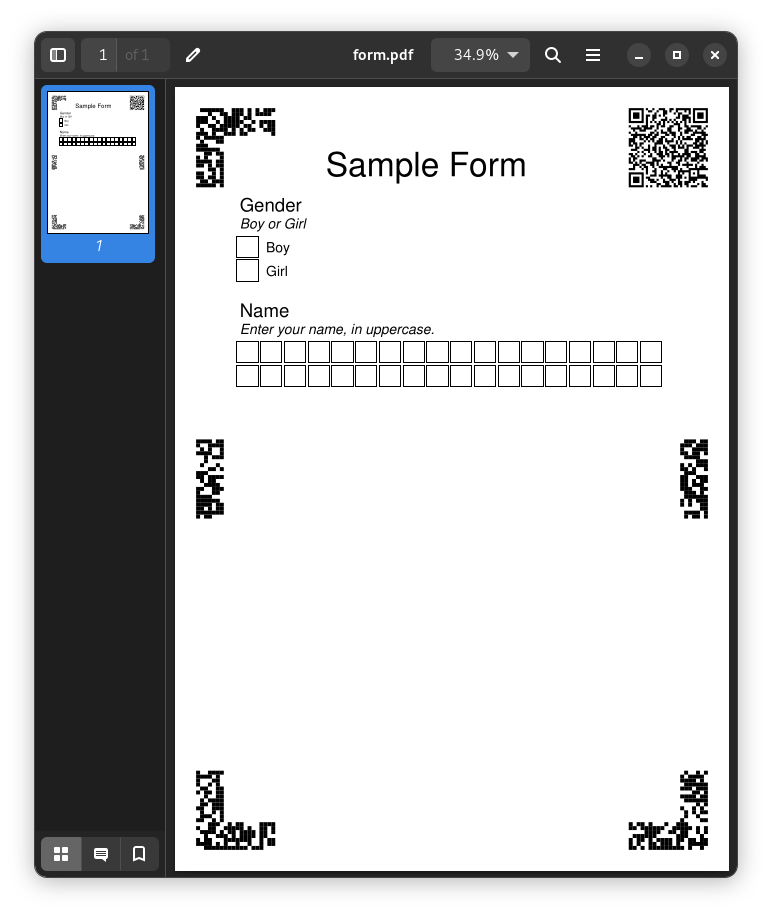
\includegraphics[height=5cm]{images/sample_form.png}
%			\caption{UML Diagram Of SmartForms's Backend Modules}
%			\label{smart-forms-modules}
		\end{figure}
		
	\end{columns}
	xcfs dkjl sdfjsd jkdfsl jsdkl jdskf jkdsf kjldsjf dskljf dskl jksdl jds jdsjkl jdsklj sdlkjf fjdksl lfjks
\end{frame}


\section{First section}

%---------------------------------------------------------
%Changing visivility of the text
\begin{frame}
	\frametitle{Sample frame title}
	This is a text in second frame. For the sake of showing an example.
	
	\begin{itemize}
		\item<1-> Text visible on slide 1
		\item<2-> Text visible on slide 2
		\item<3> Text visible on slides 3
		\item<4-> Text visible on slide 4
	\end{itemize}
\end{frame}

%---------------------------------------------------------


%---------------------------------------------------------
%Example of the \pause command
\begin{frame}
	In this slide \pause
	
	the text will be partially visible \pause
	
	And finally everything will be there
\end{frame}
%---------------------------------------------------------

\section{Second section}

%---------------------------------------------------------
%Highlighting text
\begin{frame}
	\frametitle{Sample frame title}
	
	In this slide, some important text will be
	\alert{highlighted} because it's important.
	Please, don't abuse it.
	
	\begin{block}{Remark}
		Sample text
	\end{block}
	
	\begin{alertblock}{Important theorem}
		Sample text in red box
	\end{alertblock}
	
	\begin{examples}
		Sample text in green box. The title of the block is ``Examples".
	\end{examples}
\end{frame}
%---------------------------------------------------------


%---------------------------------------------------------
%Two columns
\begin{frame}
	\frametitle{Two-column slide}
	
	\begin{columns}
		
		\column{0.5\textwidth}
		This is a text in first column.
		$$E=mc^2$$
		\begin{itemize}
			\item First item
			\item Second item
		\end{itemize}
		
		\column{0.5\textwidth}
		This text will be in the second column
		and on a second tought this is a nice looking
		layout in some cases.
	\end{columns}
\end{frame}
%---------------------------------------------------------


\end{document}